\section{Devices framework measurement offset with RIOT OS}

We notice that the mesures distributions with RIOT are the same between the reference values and the devices framework mesures.
However, the distributions are shifted to the left by an offset as shown by the figure \ref{fig:devices-comparison-riot}.
With the RE-Mote board this offset is $1.35 \mu s$ and with the Z1 board, it is $2.99 \mu s$.

\begin{figure}[!ht]
  \centering
  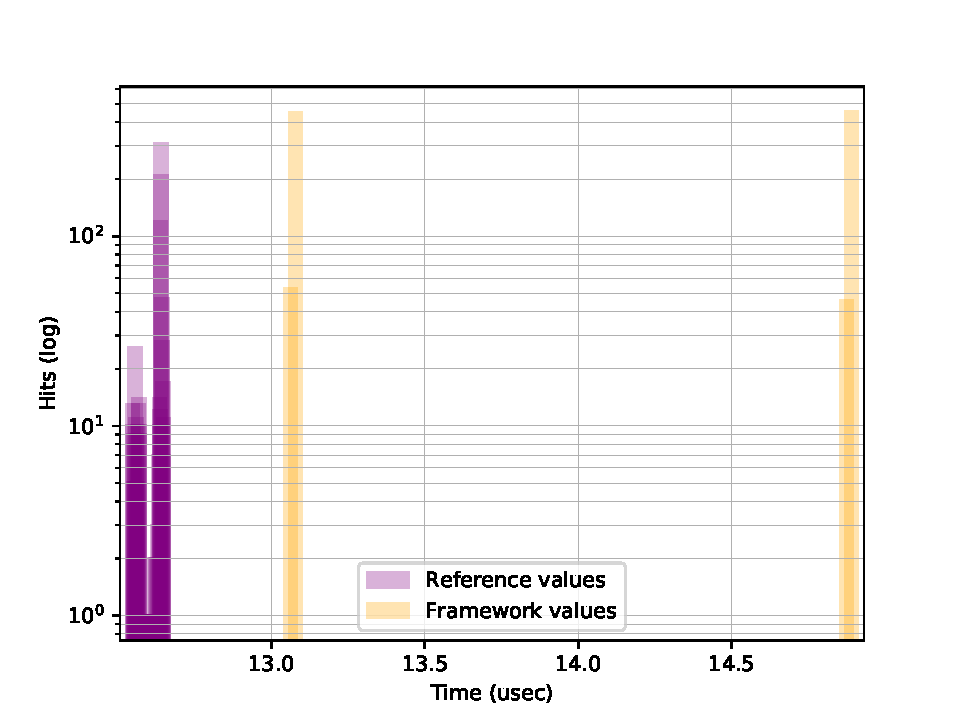
\includegraphics[scale=.7]{assets/comparison-devices-framework-riot-remote.pdf}
  \caption*{Measurements made on the RE-Mote board}
% \end{figure}

% \begin{figure}[!ht]
  \centering
  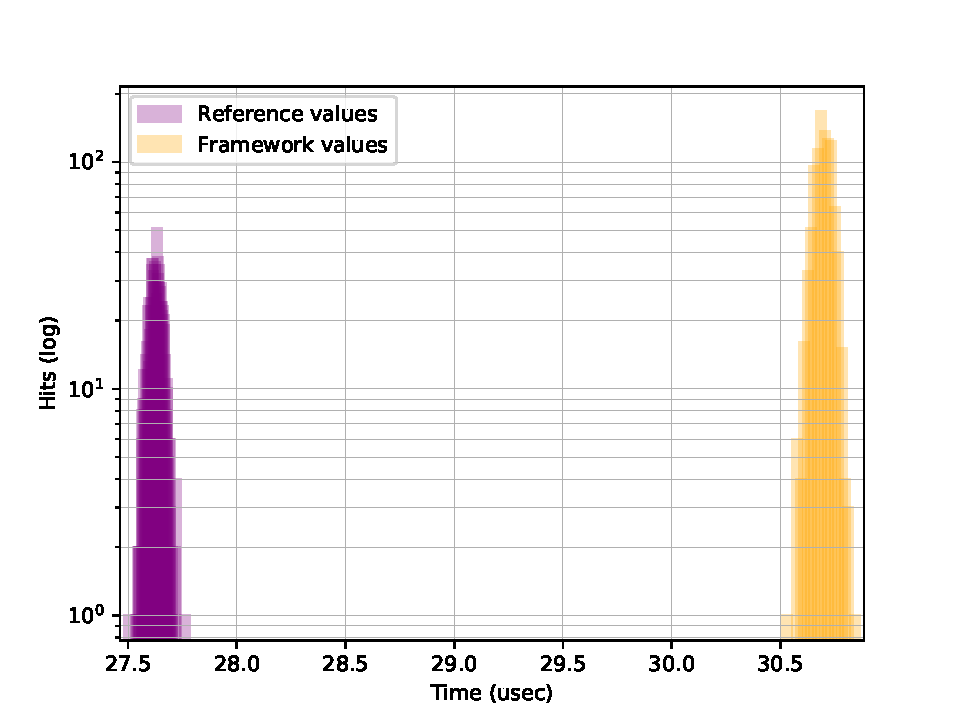
\includegraphics[scale=.7]{assets/comparison-devices-framework-riot-z1.pdf}
  \caption*{Measurements made on the Z1 board}
  \caption{comparison of the devices framework with the reference value on RIOT\label{fig:devices-comparison-riot}}
\end{figure}

\subsection{Causes}

Those offsets can be correlated with the measured overheads.
Indeed, the overheads mesured in the section \ref{sec:overhead} are the same as the offset with RIOT on the two boards.
Our hypothesis is that, with RIOT, there is hidden calls between the user space and the framework space.